\documentclass{article}
\usepackage{tabularx,ragged2e,booktabs,caption}
\usepackage{graphicx}
\usepackage{float}
\usepackage{array}
\usepackage{amsmath}

\title{Assignment 1}
\author{Francesco Andreuzzi}
\date{\today}

\begin{document}
\maketitle

\section{MPI Programming}

\subsection{Ring}

\subsubsection{Implementation}
I implemented in C++ a ring with the given characteristics. Communications are carried out using the asynchronous operations \texttt{MPI\_Isend, MPI\_Irecv}, after two input communications and two output communications on a given process the function \texttt{MPI\_Waitall} is called in order to wait for the communication to be completed. The time is measured on the process \texttt{rank0}, and I called \texttt{MPI\_Barrier} just before measuring the elapsed time in order to wait for all the other processes to receive their initial messages, which for my understanding of the problem represents the total time. Since the times I measured are quite small I repeated the experiment about 10000 times for all the parameters available.

\subsubsection{Analysis}
In Figure \ref{fig:ring_performance} we report the performance of \texttt{ring.cpp} for varying number of processors. We expect an approximately linear growth, since the addition of a new process introduces a new step in the ring (and therefore two more input and two output messages for each process).

\begin{figure}[t]
    \centering
    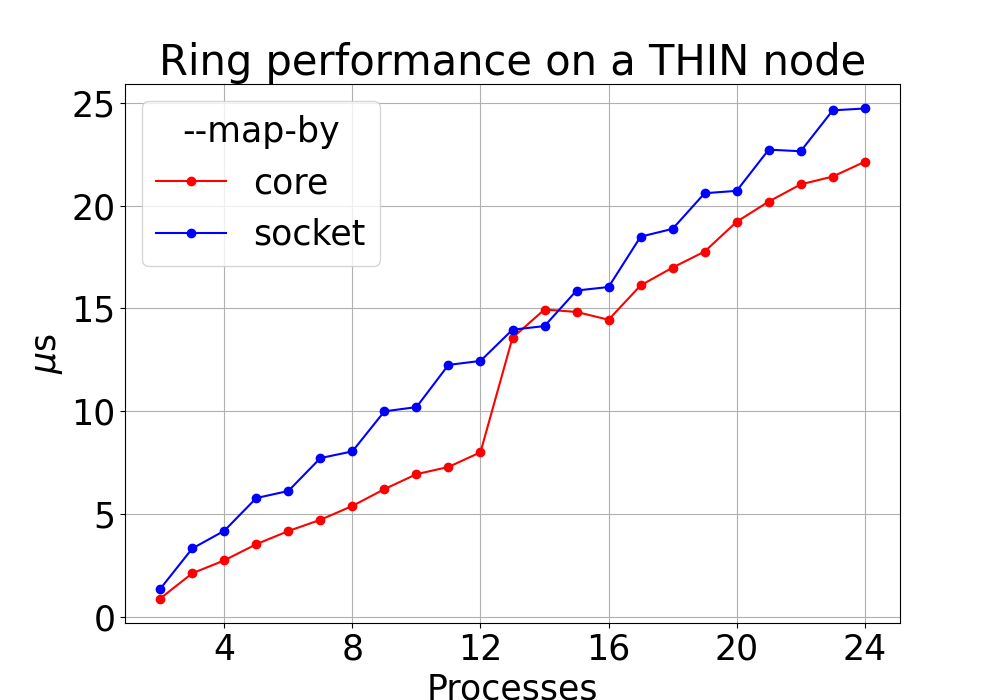
\includegraphics[width=\textwidth]{ring/fig.png}
    \caption{The script (written in C++) has been run multiple times ($\sim$ 10000) on a THIN node. Output was disabled via a compiler flag while taking times, in order to avoid polluting measurements.}
    \label{fig:ring_performance}
\end{figure}

The time is taken for two values of \texttt{--map-by}, namely \texttt{core} and \texttt{socket}. As expected the \texttt{--map-by core} case outperforms the other one until \texttt{P=13}. As soon as this threshold is passed two new communication channels are created between a process from \texttt{socket0} and a process from \texttt{socket1} (i.e. bewteen \texttt{rank11} and \texttt{rank12}, and between \texttt{rankP-1} and \texttt{rank0}), which is more costly than the communications we had in the region in the left part of the figure. However the evolution of the time recovers its linearity after the central region.

As you can see in the figure, the time taken by the \texttt{--map-by socket} case increases significantly only when the number of processors increases by 2, and is therefore slightly non-linear. For instance, when $P=7$ and $P=8$ the script takes $\sim$ 7.5 $\mu$s, but when $P=9$ it takes $\sim$10 $\mu$s. This is due to the fact that the mapping we chose for this case maps a process to \texttt{socket0} or \texttt{socket1} depending on its \texttt{rank}. Therefore the communication between \texttt{rank0} and \texttt{rankP-1} becomes more costly (i.e. involves two different sockets) when two processes are introduced; otherwise the new communication channel is quite cheap with respect to the other communications, since it occurs within the same socket.

\subsection{Matrix-Matrix addition}
The original formulation of this exercise led to a very inefficient solution for the following reason: processing rectangular sub-blocks taken from the matrix in each process required a copy in the general case, since in most cases it is not possible to have the required cells in a contiguous array (\texttt{MPI\_Scatterv} allows to increase slightly the number of treatable cases, but still does not solve the general problem). For this reason a copy before calling \texttt{MPI\_Scatter} and after calling \texttt{MPI\_Gather} is needed, thus annihilating the computational time we saved introducing MPI in the equation.

For this reason we dropped the comparison of different 1D/2D/3D topologies, and studied the \emph{strong scalability} of the summation of two 3D matrices with $P$ processes. We use \texttt{MPI\_Scatter} to send $P$ slices of size $N/P$, one for each process. Note that those slices are not blocks in the sense designated in the assignment statement: in a 3D space we could visualize them as faces of the cube (moving along the first axis). These faces may not be complete, and more than one face may be sent to each process depending on $P$ and $N$.

\textbf{Note}: I also implemented a solution for the problem which follows closely the original statement of the problem, and am able to produce it in a matter of minutes if requested.

\subsection{Experimental results}
\begin{figure}[b!]
    \centering
    \includegraphics[width=\textwidth]{matrix/time.png}
    \caption{Time measured for the addition of two 3D matrices (size $2400\times 100\times 100$). In the image we highlighted the incidence of communication time on the total time (black dotted line). The straight line at 0.05 seconds is the time it took to run the serial version of the addition (no communication).}
    \label{fig:matrix_performance}
\end{figure}

We may approximate the total time taken by the parallel implementation of the 3D matrices addition in the following way (keeping the size of the matrix fixed at $2400\times 100\times 100$):
\begin{gather}\label{eq:matrix_time_equation}
    T(P) = T_s(P) + T_\text{add}(P) + T_g(P)
\end{gather}
Where $T_s(P), T_g(P)$ are respectively the time taken by \texttt{MPI\_Scatter} and \texttt{MPI\_Gather} on $P$ processors, while $T_\text{add}(P)$ is the time taken by the summation of the portion of matrix sent to one of the $P$ processors (which may be considered approximately equal for all the processors). Obviously $T_s(1) = T_g(1) = 0$.

In Figure \ref{fig:matrix_performance} we show the contribution of each component to the total time (red dotted line). $T_\text{add}$ is the vertical distance in the plot between the total time and the communication time (black dotted line). As you can see $T_\text{add}$ is the smallest contribution, and is monotonically decreasing as expected.

By contrast, $T_s$ behaves in an unexpected way. It would make sense that the time taken by the two calls to \texttt{MPI\_Scatter} (one for each matrix to sum) increases linearly on the number of processes. However this is not the case in the left region of the plot, while we have an approximately linear relation in the right part. This probably happens due to the fact that \texttt{MPI\_Scatter} behaves in different ways depending on the number of processes and on the size of the message to send. In some cases \texttt{MPI\_Scatter} builds a binomial tree (having the root process as its root) and delegates to its child a reduced amount of work.

\section{Measure MPI point to point performance}
In this section we briefly disucss and present the results obtained with the \emph{PingPong} benchmark on Orfeo. The banchmark has been ran on multiple kind of nodes and networks, and against different implementations of MPI. Due to the variability that is usually experienced in two consecutive runs of the benchmark we repeated each experiment 1000 times, and averaged the results for element-wise.

\subsection{Differences observed between IntelMPI and OpenMPI}
Experiments with the \emph{PingPong} benchmark have been carried out using two different implementations of MPI available on \emph{Orfeo}, namely IntelMPI and OpenMPI. The time measured for 30 messages of growing size are shown in Figure \ref{fig:ompi_vs_intel}. It is clear that the main difference is that IntelMPI looks much more stable than OpenMPI, especially in the left region. Since the interested region is the one in which latency is dominant with respect to the bandwidth, we may assume that the two implementations communicate in different ways with the network interface, thus encountering different costs in establishing the communication and sending the message.

\begin{figure}[t]
    \centering
    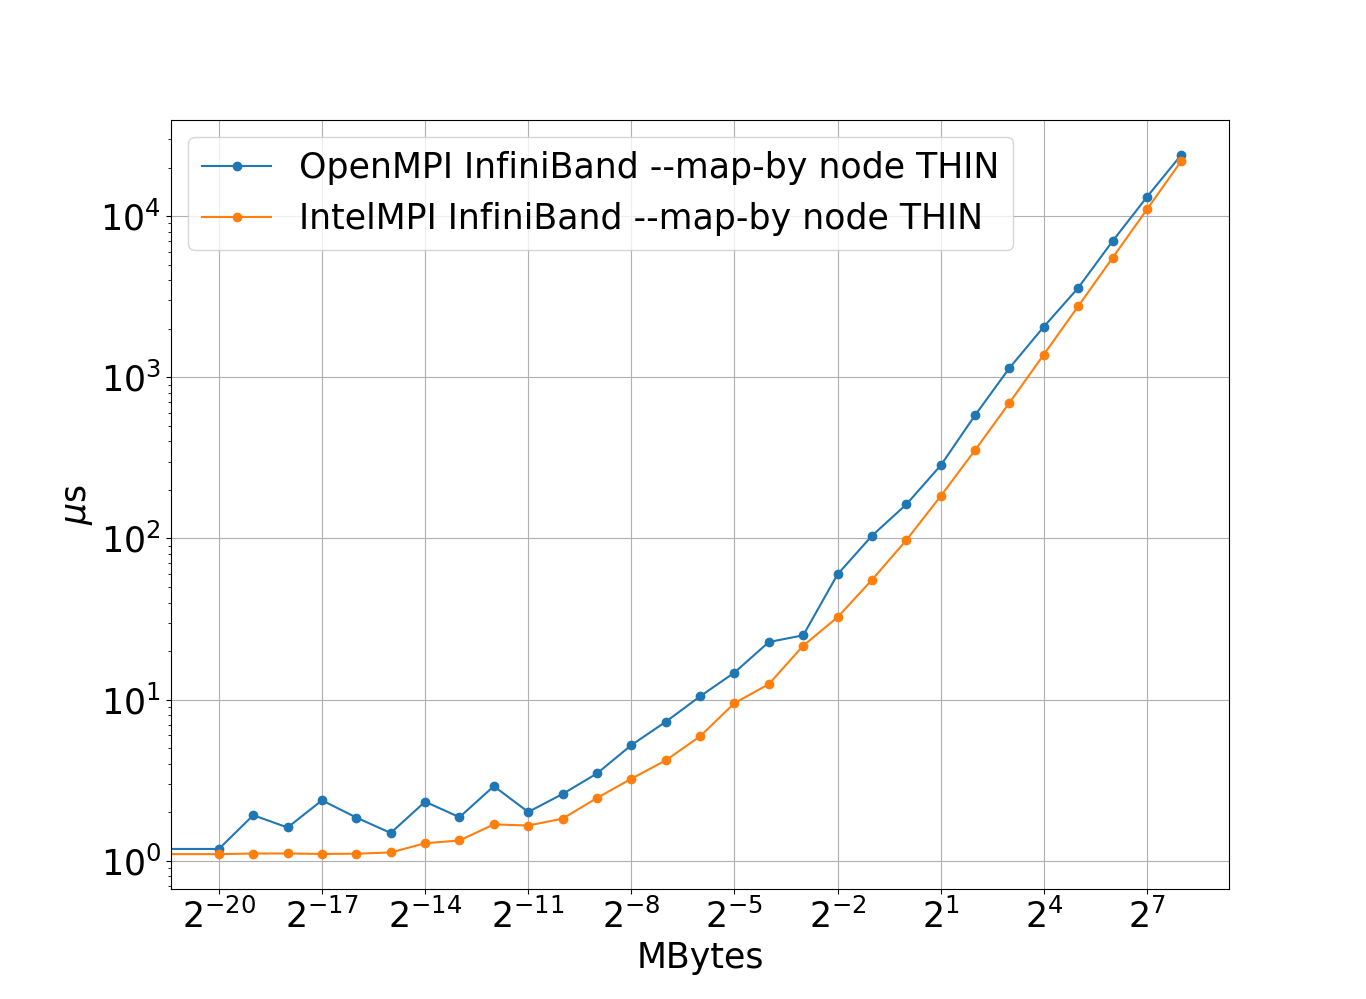
\includegraphics[width=\textwidth]{benchmark/intel_vs_ompi_node.png}
    \caption{Comparison of the time measured during the \emph{PingPong} benchmark using IntelMPI and OpenMPI, \emph{InfiniBand}, on two THIN nodes.}
    \label{fig:ompi_vs_intel}
\end{figure}

\begin{figure}[b]
    $$
        \begin{array}{c | c | c} \hline
            & \text{OpenMPI} & \text{IntelMPI} \\ \hline
            \hline
            \text{Core} & 0.2 \mu \text{s}  & 0.23 \mu \text{s} \\ \hline
            \text{Socket} & 0.4 \mu \text{s}  & 0.42 \mu \text{s} \\ \hline
            \text{Node} & 1.58 \mu \text{s}  & 1.08 \mu \text{s} \\ \hline
        \end{array}
    $$
    \caption{Latency computed using the simplified linear network module in OpenMPI and IntelMPI (using \emph{InfiniBand}, on THIN nodes).}
    \label{tab:lat_ompi_intel}
\end{figure}

This assumption is supported also by the latency computed using the simplified network model (Table \ref{tab:lat_ompi_intel}), which is substantially different if we switch the MPI implementation.

\subsection{Differences observed between Infiniband and Gigabit}
\begin{figure}[t]
    \centering
    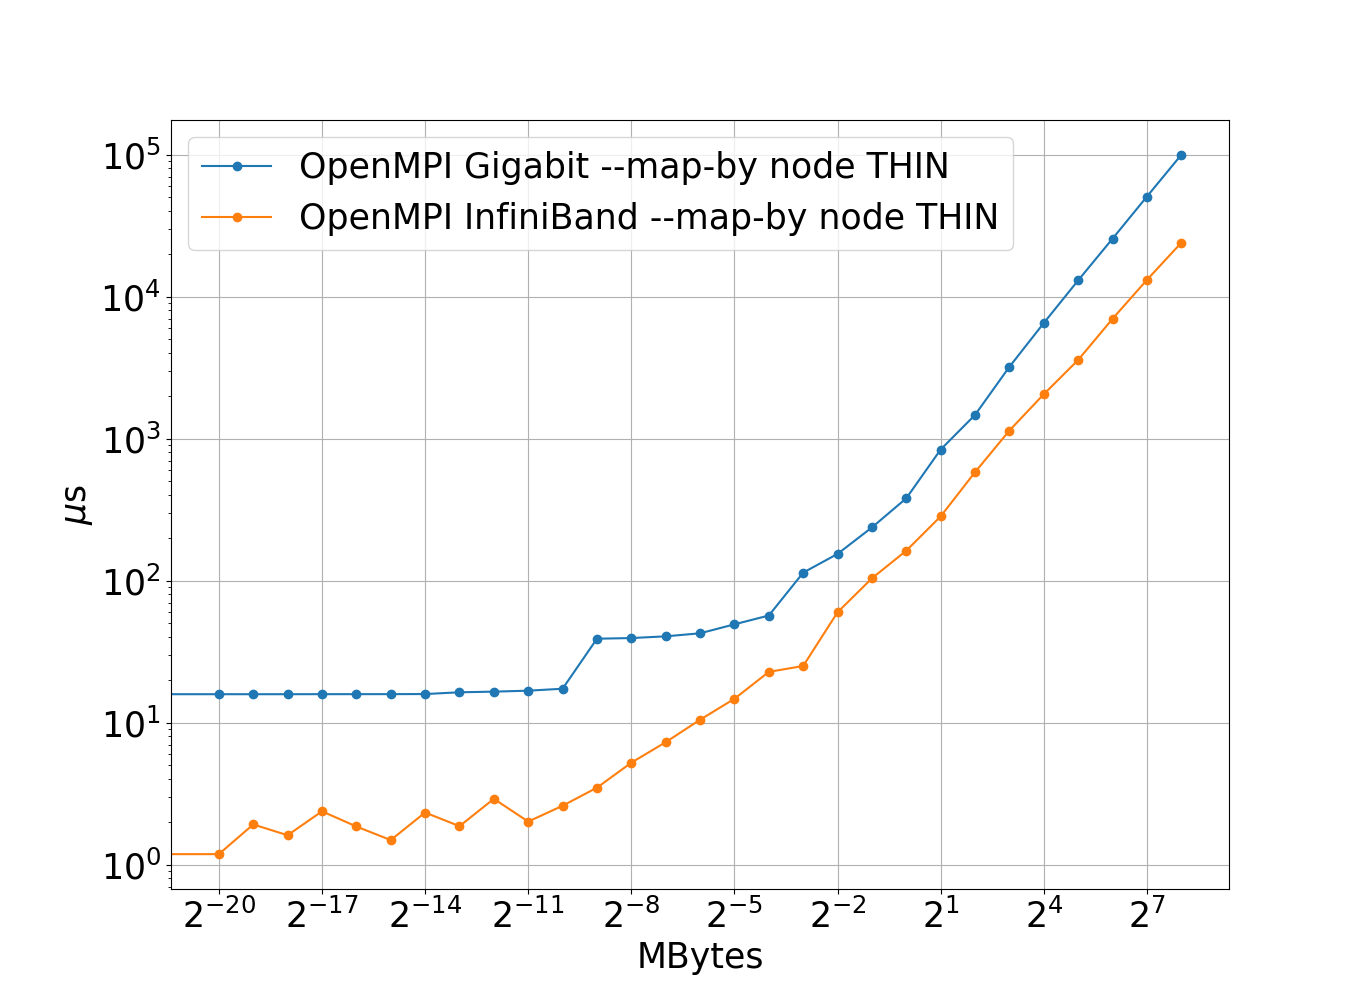
\includegraphics[width=\textwidth]{benchmark/infi_vs_giga_node.png}
    \caption{Comparison of the time measured with the \emph{PingPong} benchmark using InfiniBand and Gigabit network with OpenMPI, on two THIN nodes.}
    \label{fig:infi_vs_giga}
\end{figure}

Looking at the left region of the graph shown in Figure \ref{fig:infi_vs_giga}, we see that the latency is clearly very different in the two cases. This is most likely due to the fact that the Gigabit network performs some more controls on the communication (e.g. it verifies that the message arrives to the receiver), therefore the message needs to pass through more layers with respect to InfiniBand network. Also, InfiniBand employs several "tricks" to make the communication faster, which likely contributes to the reduced latency. For instance when using Gigabit the user of the network has to pre-process the message using its own computational resources. This does not happen with InfiniBand, since the pre-processing happens on a software module of the network.

\begin{figure}[t]
    \centering
    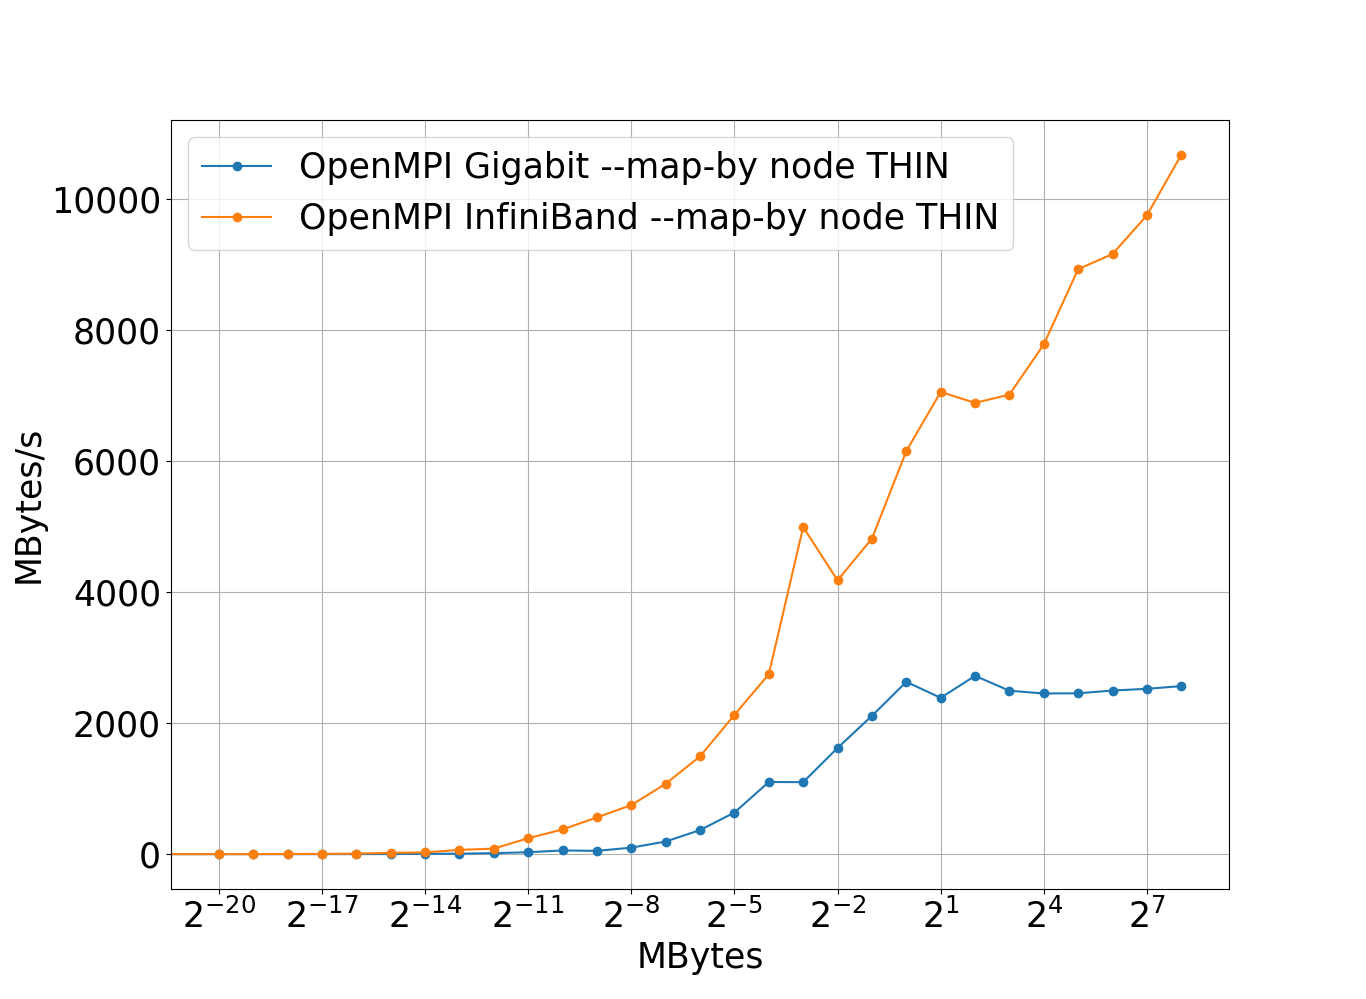
\includegraphics[width=\textwidth]{benchmark/infi_vs_giga_node_bandw.png}
    \caption{Comparison of the bandwidth measured with the \emph{PingPong} benchmark using InfiniBand and Gigabit network with OpenMPI, on two THIN nodes.}
    \label{fig:infi_vs_giga_bandwidth}
\end{figure}

Also, as you can see in Figure \ref{fig:infi_vs_giga_bandwidth}, the asymptotic bandwidth is much higher when we use InfiniBand, which is something that we could have expected before-hand.

\subsection{Other observations}
\begin{figure}[t]
    \centering
    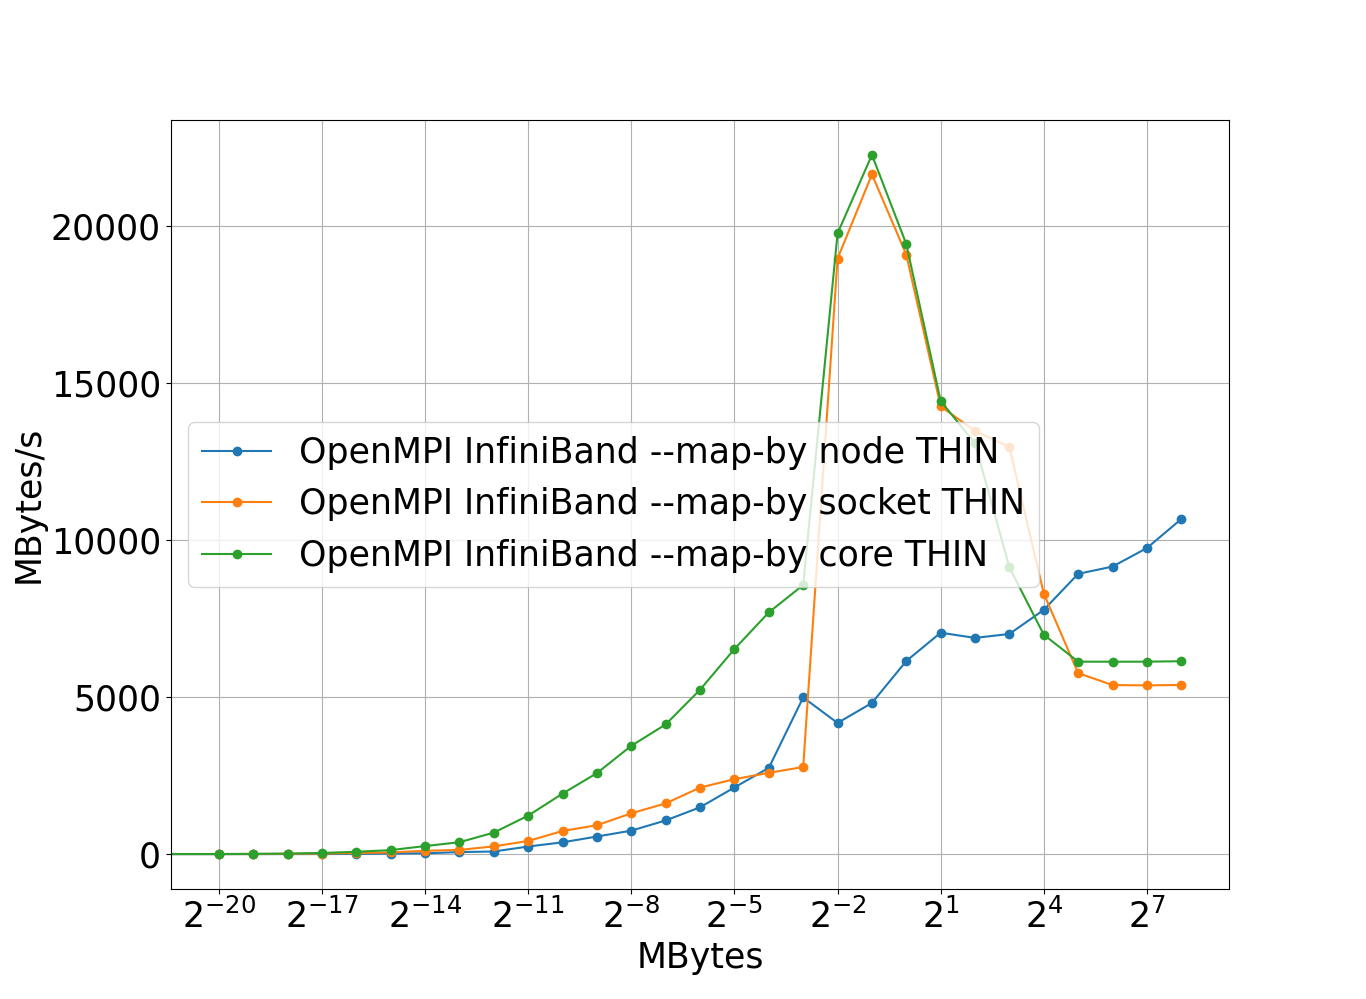
\includegraphics[width=\textwidth]{benchmark/mapby_bandwidth.png}
    \caption{Comparison of the bandwidth measured with the \emph{PingPong} benchmark using different distributions of the processes (same core, different sockets, different nodes) with OpenMPI, on THIN nodes.}
    \label{fig:mapby}
\end{figure}

No substantial differences have been observed between THIN and GPU nodes, using both IntelMPI and OpenMPI.

It is interesting to observe that the measured asymptotic bandwidth is higher when the processes live in different nodes, than the bandwidth measured when the processes are on the same node. However the maximum bandwidth achieved is reached only in the latter case. An hypothesis which may be proposed is that this happens due to how the message is delivered in the two cases:
\begin{itemize}
    \item When the processes live in different nodes, the message is delivered using InfiniBand network, which results in the asymptotic bandwidth observed above;
    \item When the processes live in the same node the message is delivered using the shared layers of cache (we have more shared layers if the processes are in the same socket, see the case \texttt{--map-by core} in Figure \ref{fig:mapby}).
\end{itemize}
The parts of the graphs in which we see a decrease, if this hypothesis is correct, are the regions in which the current message size does not fit into the cache level which was used up to this moment, therefore the time needed to transfer the message from now on is higher. Asymptotically, the message does not fit into any cache level.

\section{Compare performance observed against performance model for Jacobi solver}

\begin{figure}
    $$
        \begin{array}{c | c | c | c | c | c | c | c | c} \hline
            N  & Nx & Ny & Nz & k & C(L,N)  & T_c(L,N) &     P(L,N)     & \frac{P(1)*N}{P(L,N)} \\ \hline
            \hline
            4  & 2  & 2  & 1  & 4 & 87.891  &  0.014   & 456.775  &         0.989         \\ \hline
            8  & 2  & 2  & 2  & 6 & 131.836 &  0.022   & 913.115  &         0.989         \\ \hline
            12 & 3  & 2  & 2  & 6 & 131.836 &  0.022   & 1369.673 &         0.989         \\ \hline
        \end{array}
    $$
    \caption{One thin node, \texttt{--map-by core}, latency: 0.19 $\mu$s, bandwidth: 6095 MB/s.}
\end{figure}


\begin{figure}
    $$
        \begin{array}{c | c | c | c | c | c | c | c | c} \hline
            N  & Nx & Ny & Nz & k & C(L,N)  & T_c(L,N) &     P(L,N)     & \frac{P(1)*N}{P(L,N)} \\ \hline
            \hline
            4  & 2  & 2  & 1  & 4 & 87.891  &  0.017   & 456.711  &         0.989         \\ \hline
            8  & 2  & 2  & 2  & 6 & 131.836 &  0.025   & 912.922  &         0.989         \\ \hline
            12 & 3  & 2  & 2  & 6 & 131.836 &  0.025   & 1369.383 &         0.989         \\ \hline
        \end{array}
    $$
    \caption{One thin node, \texttt{--map-by socket}, latency: 0.4 $\mu$s, bandwidth: 5307 MB/s.}
\end{figure}


\begin{figure}
    $$
        \begin{array}{c | c | c | c | c | c | c | c | c} \hline
            N  & Nx & Ny & Nz & k & C(L,N)  & T_c(L,N) &     P(L,N)     & \frac{P(1)*N}{P(L,N)} \\ \hline
            \hline
            12 & 3  & 2  & 2  & 6 & 131.836 &  0.012   & 953.944  &         0.985         \\ \hline
            24 & 4  & 3  & 2  & 6 & 131.836 &  0.012   & 1907.887 &         0.985         \\ \hline
            48 & 4  & 4  & 3  & 6 & 131.836 &  0.012   & 3815.774 &         0.985         \\ \hline
        \end{array}
    $$
    \caption{Two thin nodes, latency: 1.58 $\mu$s, bandwidth: 10670 MB/s.}
\end{figure}


\begin{figure}
    $$
        \begin{array}{c | c | c | c | c | c | c | c | c} \hline
            N  & Nx & Ny & Nz & k & C(L,N)  & T_c(L,N) &     P(L,N)     & \frac{P(1)*N}{P(L,N)} \\ \hline
            \hline
            12 & 3  & 2  & 2  & 6 & 131.836 &   0.03   & 1368.929 &         0.99          \\ \hline
            24 & 4  & 3  & 2  & 6 & 131.836 &   0.03   & 2737.858 &         0.99          \\ \hline
            48 & 4  & 4  & 3  & 6 & 131.836 &   0.03   & 5475.716 &         0.99          \\ \hline
        \end{array}
    $$
    \caption{GPU node, hyperthreading enabled, latency: 0.43 $\mu$s, bandwidth: 4415 MB/s.}
\end{figure}

\end{document}
